\documentclass[1p]{elsarticle_modified}
%\bibliographystyle{elsarticle-num}

%\usepackage[colorlinks]{hyperref}
%\usepackage{abbrmath_seonhwa} %\Abb, \Ascr, \Acal ,\Abf, \Afrak
\usepackage{amsfonts}
\usepackage{amssymb}
\usepackage{amsmath}
\usepackage{amsthm}
\usepackage{scalefnt}
\usepackage{amsbsy}
\usepackage{kotex}
\usepackage{caption}
\usepackage{subfig}
\usepackage{color}
\usepackage{graphicx}
\usepackage{xcolor} %% white, black, red, green, blue, cyan, magenta, yellow
\usepackage{float}
\usepackage{setspace}
\usepackage{hyperref}

\usepackage{tikz}
\usetikzlibrary{arrows}

\usepackage{multirow}
\usepackage{array} % fixed length table
\usepackage{hhline}

%%%%%%%%%%%%%%%%%%%%%
\makeatletter
\renewcommand*\env@matrix[1][\arraystretch]{%
	\edef\arraystretch{#1}%
	\hskip -\arraycolsep
	\let\@ifnextchar\new@ifnextchar
	\array{*\c@MaxMatrixCols c}}
\makeatother %https://tex.stackexchange.com/questions/14071/how-can-i-increase-the-line-spacing-in-a-matrix
%%%%%%%%%%%%%%%

\usepackage[normalem]{ulem}

\newcommand{\msout}[1]{\ifmmode\text{\sout{\ensuremath{#1}}}\else\sout{#1}\fi}
%SOURCE: \msout is \stkout macro in https://tex.stackexchange.com/questions/20609/strikeout-in-math-mode

\newcommand{\cancel}[1]{
	\ifmmode
	{\color{red}\msout{#1}}
	\else
	{\color{red}\sout{#1}}
	\fi
}

\newcommand{\add}[1]{
	{\color{blue}\uwave{#1}}
}

\newcommand{\replace}[2]{
	\ifmmode
	{\color{red}\msout{#1}}{\color{blue}\uwave{#2}}
	\else
	{\color{red}\sout{#1}}{\color{blue}\uwave{#2}}
	\fi
}

\newcommand{\Sol}{\mathcal{S}} %segment
\newcommand{\D}{D} %diagram
\newcommand{\A}{\mathcal{A}} %arc


%%%%%%%%%%%%%%%%%%%%%%%%%%%%%5 test

\def\sl{\operatorname{\textup{SL}}(2,\Cbb)}
\def\psl{\operatorname{\textup{PSL}}(2,\Cbb)}
\def\quan{\mkern 1mu \triangleright \mkern 1mu}

\theoremstyle{definition}
\newtheorem{thm}{Theorem}[section]
\newtheorem{prop}[thm]{Proposition}
\newtheorem{lem}[thm]{Lemma}
\newtheorem{ques}[thm]{Question}
\newtheorem{cor}[thm]{Corollary}
\newtheorem{defn}[thm]{Definition}
\newtheorem{exam}[thm]{Example}
\newtheorem{rmk}[thm]{Remark}
\newtheorem{alg}[thm]{Algorithm}

\newcommand{\I}{\sqrt{-1}}
\begin{document}

%\begin{frontmatter}
%
%\title{Boundary parabolic representations of knots up to 8 crossings}
%
%%% Group authors per affiliation:
%\author{Yunhi Cho} 
%\address{Department of Mathematics, University of Seoul, Seoul, Korea}
%\ead{yhcho@uos.ac.kr}
%
%
%\author{Seonhwa Kim} %\fnref{s_kim}}
%\address{Center for Geometry and Physics, Institute for Basic Science, Pohang, 37673, Korea}
%\ead{ryeona17@ibs.re.kr}
%
%\author{Hyuk Kim}
%\address{Department of Mathematical Sciences, Seoul National University, Seoul 08826, Korea}
%\ead{hyukkim@snu.ac.kr}
%
%\author{Seokbeom Yoon}
%\address{Department of Mathematical Sciences, Seoul National University, Seoul, 08826,  Korea}
%\ead{sbyoon15@snu.ac.kr}
%
%\begin{abstract}
%We find all boundary parabolic representation of knots up to 8 crossings.
%
%\end{abstract}
%\begin{keyword}
%    \MSC[2010] 57M25 
%\end{keyword}
%
%\end{frontmatter}

%\linenumbers
%\tableofcontents
%
\newcommand\colored[1]{\textcolor{white}{\rule[-0.35ex]{0.8em}{1.4ex}}\kern-0.8em\color{red} #1}%
%\newcommand\colored[1]{\textcolor{white}{ #1}\kern-2.17ex	\textcolor{white}{ #1}\kern-1.81ex	\textcolor{white}{ #1}\kern-2.15ex\color{red}#1	}

{\Large $\underline{11n_{150}~(K11n_{150})}$}

\setlength{\tabcolsep}{10pt}
\renewcommand{\arraystretch}{1.6}
\vspace{1cm}\begin{tabular}{m{100pt}>{\centering\arraybackslash}m{274pt}}
\multirow{5}{120pt}{
	\centering
	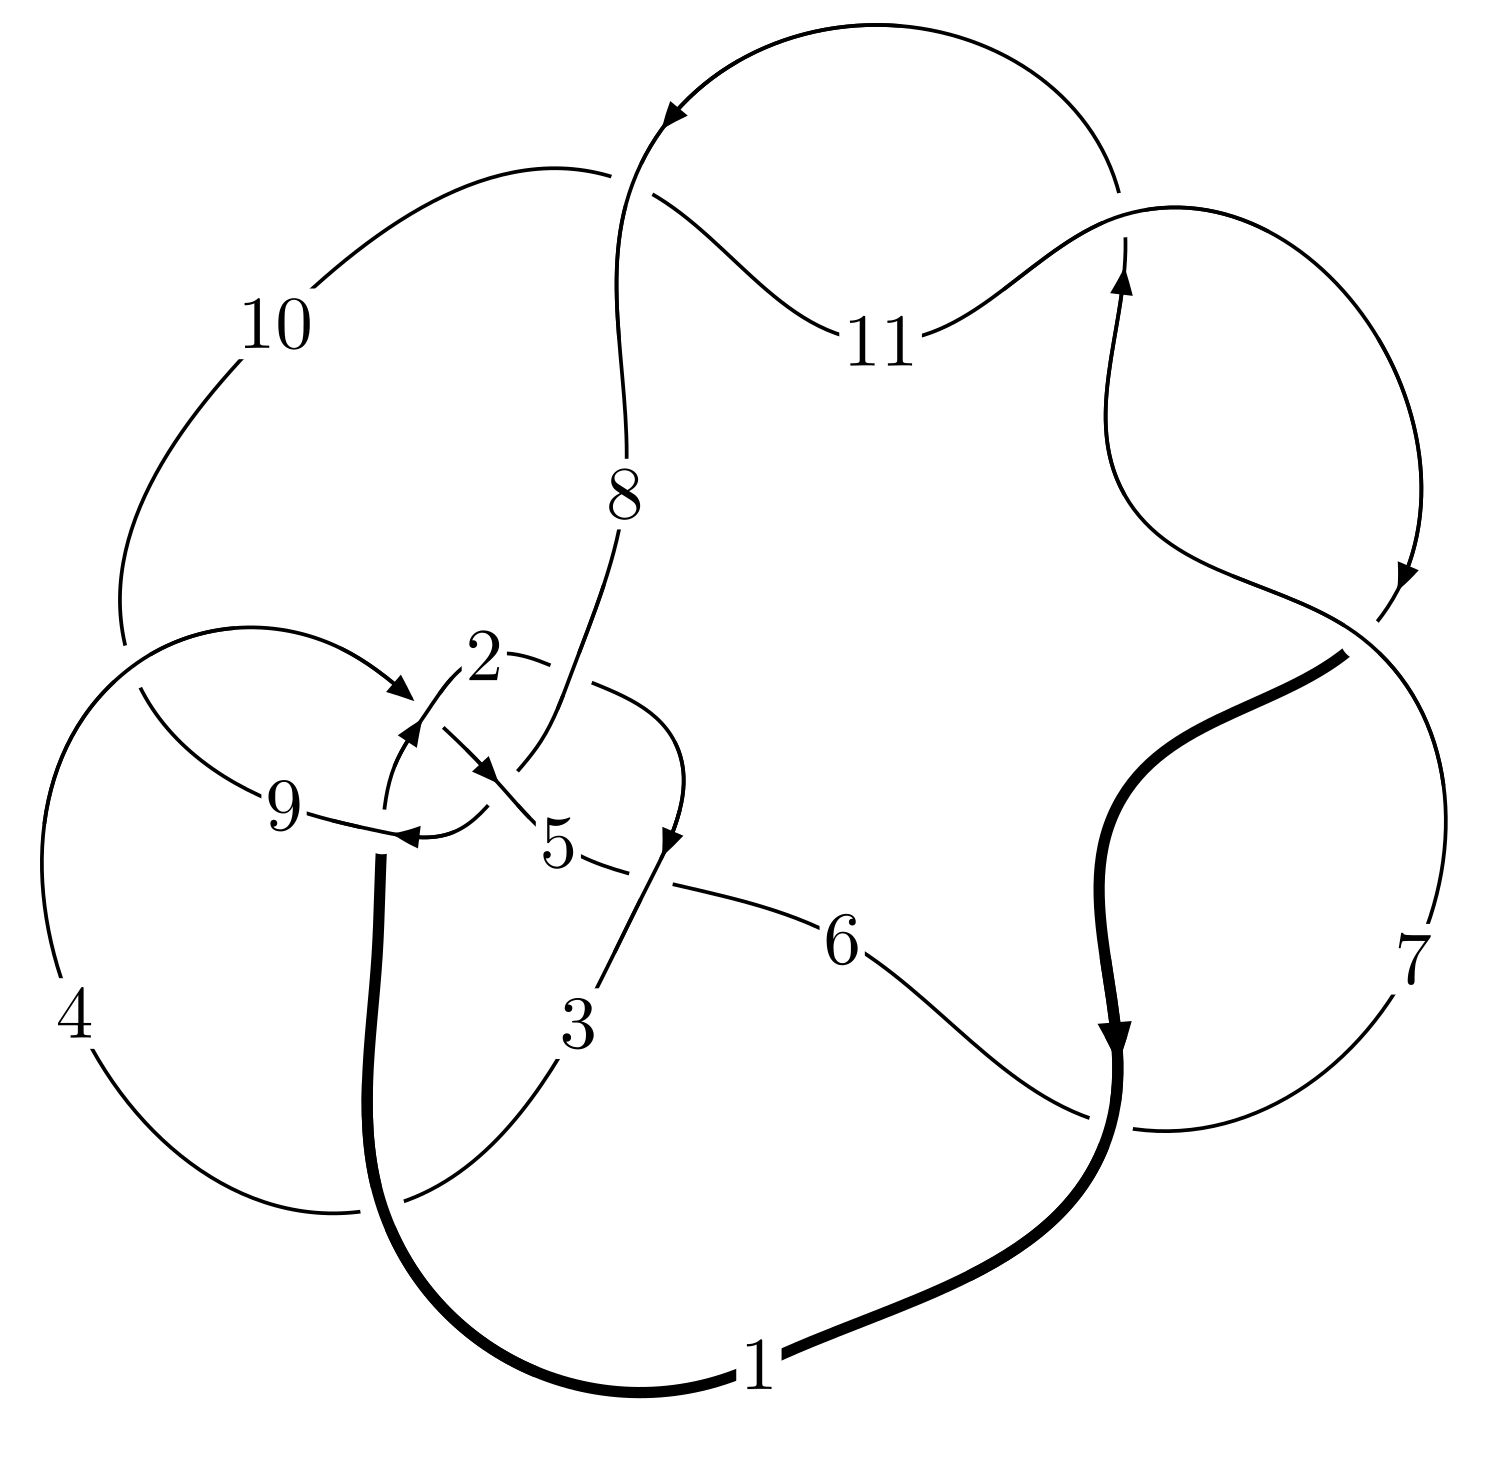
\includegraphics[width=112pt]{../../../GIT/diagram.site/Diagrams/png/766_11n_150.png}\\
\ \ \ A knot diagram\footnotemark}&
\allowdisplaybreaks
\textbf{Linearized knot diagam} \\
\cline{2-2}
 &
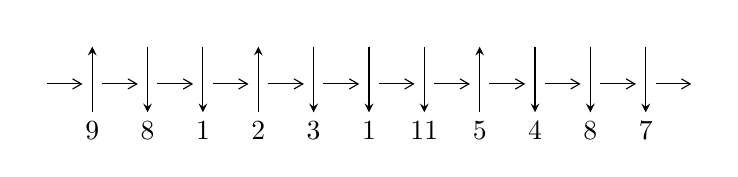
\begin{tikzpicture}[x=20pt, y=17pt]
	% nodes
	\node (C0) at (0, 0) {};
	\node (C1) at (1, 0) {};
	\node (C1U) at (1, +1) {};
	\node (C1D) at (1, -1) {9};

	\node (C2) at (2, 0) {};
	\node (C2U) at (2, +1) {};
	\node (C2D) at (2, -1) {8};

	\node (C3) at (3, 0) {};
	\node (C3U) at (3, +1) {};
	\node (C3D) at (3, -1) {1};

	\node (C4) at (4, 0) {};
	\node (C4U) at (4, +1) {};
	\node (C4D) at (4, -1) {2};

	\node (C5) at (5, 0) {};
	\node (C5U) at (5, +1) {};
	\node (C5D) at (5, -1) {3};

	\node (C6) at (6, 0) {};
	\node (C6U) at (6, +1) {};
	\node (C6D) at (6, -1) {1};

	\node (C7) at (7, 0) {};
	\node (C7U) at (7, +1) {};
	\node (C7D) at (7, -1) {11};

	\node (C8) at (8, 0) {};
	\node (C8U) at (8, +1) {};
	\node (C8D) at (8, -1) {5};

	\node (C9) at (9, 0) {};
	\node (C9U) at (9, +1) {};
	\node (C9D) at (9, -1) {4};

	\node (C10) at (10, 0) {};
	\node (C10U) at (10, +1) {};
	\node (C10D) at (10, -1) {8};

	\node (C11) at (11, 0) {};
	\node (C11U) at (11, +1) {};
	\node (C11D) at (11, -1) {7};
	\node (C12) at (12, 0) {};

	% arrows
	\draw[->,>={angle 60}]
	(C0) edge (C1) (C1) edge (C2) (C2) edge (C3) (C3) edge (C4) (C4) edge (C5) (C5) edge (C6) (C6) edge (C7) (C7) edge (C8) (C8) edge (C9) (C9) edge (C10) (C10) edge (C11) (C11) edge (C12) ;	\draw[->,>=stealth]
	(C1D) edge (C1U) (C2U) edge (C2D) (C3U) edge (C3D) (C4D) edge (C4U) (C5U) edge (C5D) (C6U) edge (C6D) (C7U) edge (C7D) (C8D) edge (C8U) (C9U) edge (C9D) (C10U) edge (C10D) (C11U) edge (C11D) ;
	\end{tikzpicture} \\
\hhline{~~} \\& 
\textbf{Solving Sequence} \\ \cline{2-2} 
 &
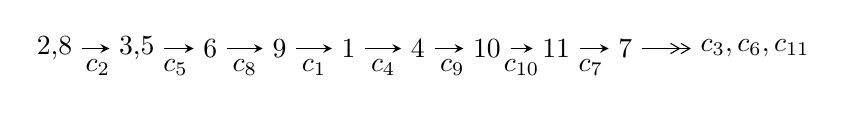
\begin{tikzpicture}[x=25pt, y=7pt]
	% node
	\node (A0) at (-1/8, 0) {2,8};
	\node (A1) at (17/16, 0) {3,5};
	\node (A2) at (17/8, 0) {6};
	\node (A3) at (25/8, 0) {9};
	\node (A4) at (33/8, 0) {1};
	\node (A5) at (41/8, 0) {4};
	\node (A6) at (49/8, 0) {10};
	\node (A7) at (57/8, 0) {11};
	\node (A8) at (65/8, 0) {7};
	\node (C1) at (1/2, -1) {$c_{2}$};
	\node (C2) at (13/8, -1) {$c_{5}$};
	\node (C3) at (21/8, -1) {$c_{8}$};
	\node (C4) at (29/8, -1) {$c_{1}$};
	\node (C5) at (37/8, -1) {$c_{4}$};
	\node (C6) at (45/8, -1) {$c_{9}$};
	\node (C7) at (53/8, -1) {$c_{10}$};
	\node (C8) at (61/8, -1) {$c_{7}$};
	\node (A9) at (10, 0) {$c_{3},c_{6},c_{11}$};

	% edge
	\draw[->,>=stealth]	
	(A0) edge (A1) (A1) edge (A2) (A2) edge (A3) (A3) edge (A4) (A4) edge (A5) (A5) edge (A6) (A6) edge (A7) (A7) edge (A8) ;
	\draw[->>,>={angle 60}]	
	(A8) edge (A9);
\end{tikzpicture} \\ 

\end{tabular} \\

\footnotetext{
The image of knot diagram is generated by the software ``\textbf{Draw programme}" developed by Andrew Bartholomew(\url{http://www.layer8.co.uk/maths/draw/index.htm\#Running-draw}), where we modified some parts for our purpose(\url{https://github.com/CATsTAILs/LinksPainter}).
}\phantom \\ \newline 
\centering \textbf{Ideals for irreducible components\footnotemark of $X_{\text{par}}$} 
 
\begin{align*}
I^u_{1}&=\langle 
2575706427464 u^{21}-75635053703013 u^{20}+\cdots+105076803822638 b-642339227026933,\\
\phantom{I^u_{1}}&\phantom{= \langle  }1743319071217019 u^{21}+1770759336218560 u^{20}+\cdots+525384019113190 a-4689968007233431,\\
\phantom{I^u_{1}}&\phantom{= \langle  }u^{22}-4 u^{20}+\cdots-14 u+5\rangle \\
I^u_{2}&=\langle 
7.75318\times10^{41} u^{23}+7.31958\times10^{41} u^{22}+\cdots+5.04425\times10^{43} b+5.71288\times10^{43},\\
\phantom{I^u_{2}}&\phantom{= \langle  }-3.32426\times10^{43} u^{23}-4.90017\times10^{43} u^{22}+\cdots+9.24779\times10^{44} a+2.28923\times10^{45},\\
\phantom{I^u_{2}}&\phantom{= \langle  }u^{24}+u^{23}+\cdots-14 u+11\rangle \\
I^u_{3}&=\langle 
- u^2+b+1,\;u^8- u^7-2 u^6+u^5+3 u^4-4 u^2+a+u+2,\;u^9-2 u^7- u^6+2 u^5+2 u^4-2 u^3- u^2+u+1\rangle \\
\\
\end{align*}
\raggedright * 3 irreducible components of $\dim_{\mathbb{C}}=0$, with total 55 representations.\\
\footnotetext{All coefficients of polynomials are rational numbers. But the coefficients are sometimes approximated in decimal forms when there is not enough margin.}
\newpage
\renewcommand{\arraystretch}{1}
\centering \section*{I. $I^u_{1}= \langle 2.58\times10^{12} u^{21}-7.56\times10^{13} u^{20}+\cdots+1.05\times10^{14} b-6.42\times10^{14},\;1.74\times10^{15} u^{21}+1.77\times10^{15} u^{20}+\cdots+5.25\times10^{14} a-4.69\times10^{15},\;u^{22}-4 u^{20}+\cdots-14 u+5 \rangle$}
\flushleft \textbf{(i) Arc colorings}\\
\begin{tabular}{m{7pt} m{180pt} m{7pt} m{180pt} }
\flushright $a_{2}=$&$\begin{pmatrix}1\\0\end{pmatrix}$ \\
\flushright $a_{8}=$&$\begin{pmatrix}0\\u\end{pmatrix}$ \\
\flushright $a_{3}=$&$\begin{pmatrix}1\\u^2\end{pmatrix}$ \\
\flushright $a_{5}=$&$\begin{pmatrix}-3.31818 u^{21}-3.37041 u^{20}+\cdots-24.1967 u+8.92674\\-0.0245126 u^{21}+0.719807 u^{20}+\cdots+0.565515 u+6.11304\end{pmatrix}$ \\
\flushright $a_{6}=$&$\begin{pmatrix}-6.91563 u^{21}-7.12434 u^{20}+\cdots-55.3570 u+19.6657\\-3.62984 u^{21}-2.30969 u^{20}+\cdots-34.0023 u+24.8827\end{pmatrix}$ \\
\flushright $a_{9}=$&$\begin{pmatrix}10.1768 u^{21}+5.97138 u^{20}+\cdots+106.076 u-77.2357\\-3.37041 u^{21}-3.62196 u^{20}+\cdots-37.5278 u+16.5909\end{pmatrix}$ \\
\flushright $a_{1}=$&$\begin{pmatrix}15.2289 u^{21}+12.3246 u^{20}+\cdots+150.786 u-83.4067\\5.97138 u^{21}+2.84888 u^{20}+\cdots+65.2393 u-50.8839\end{pmatrix}$ \\
\flushright $a_{4}=$&$\begin{pmatrix}-3.29367 u^{21}-4.09022 u^{20}+\cdots-24.7622 u+2.81370\\-0.0245126 u^{21}+0.719807 u^{20}+\cdots+0.565515 u+6.11304\end{pmatrix}$ \\
\flushright $a_{10}=$&$\begin{pmatrix}14.2670 u^{21}+10.4261 u^{20}+\cdots+149.374 u-93.7040\\-4.09022 u^{21}-4.45473 u^{20}+\cdots-43.2977 u+16.4683\end{pmatrix}$ \\
\flushright $a_{11}=$&$\begin{pmatrix}14.2670 u^{21}+10.4261 u^{20}+\cdots+149.374 u-93.7040\\2.71761 u^{21}-0.249682 u^{20}+\cdots+31.3329 u-35.6622\end{pmatrix}$ \\
\flushright $a_{7}=$&$\begin{pmatrix}5.68713 u^{21}+4.69087 u^{20}+\cdots+59.0094 u-36.8288\\-0.0869368 u^{21}+1.65095 u^{20}+\cdots-4.06164 u+14.6425\end{pmatrix}$\\ \flushright $a_{7}=$&$\begin{pmatrix}5.68713 u^{21}+4.69087 u^{20}+\cdots+59.0094 u-36.8288\\-0.0869368 u^{21}+1.65095 u^{20}+\cdots-4.06164 u+14.6425\end{pmatrix}$\\&\end{tabular}
\flushleft \textbf{(ii) Obstruction class $= -1$}\\~\\
\flushleft \textbf{(iii) Cusp Shapes $= -\frac{46675218577444}{52538401911319} u^{21}+\frac{154724488953125}{52538401911319} u^{20}+\cdots+\frac{718281907576011}{52538401911319} u+\frac{149853052606131}{52538401911319}$}\\~\\
\newpage\renewcommand{\arraystretch}{1}
\flushleft \textbf{(iv) u-Polynomials at the component}\newline \\
\begin{tabular}{m{50pt}|m{274pt}}
Crossings & \hspace{64pt}u-Polynomials at each crossing \\
\hline $$\begin{aligned}c_{1},c_{8}\end{aligned}$$&$\begin{aligned}
&u^{22}- u^{21}+\cdots- u+1
\end{aligned}$\\
\hline $$\begin{aligned}c_{2},c_{9}\end{aligned}$$&$\begin{aligned}
&u^{22}-4 u^{20}+\cdots+14 u+5
\end{aligned}$\\
\hline $$\begin{aligned}c_{3},c_{5}\end{aligned}$$&$\begin{aligned}
&u^{22}+2 u^{21}+\cdots-2 u+1
\end{aligned}$\\
\hline $$\begin{aligned}c_{4}\end{aligned}$$&$\begin{aligned}
&u^{22}+14 u^{21}+\cdots+11 u+2
\end{aligned}$\\
\hline $$\begin{aligned}c_{6},c_{7},c_{10}\\c_{11}\end{aligned}$$&$\begin{aligned}
&u^{22}-5 u^{21}+\cdots-3 u+4
\end{aligned}$\\
\hline
\end{tabular}\\~\\
\newpage\renewcommand{\arraystretch}{1}
\flushleft \textbf{(v) Riley Polynomials at the component}\newline \\
\begin{tabular}{m{50pt}|m{274pt}}
Crossings & \hspace{64pt}Riley Polynomials at each crossing \\
\hline $$\begin{aligned}c_{1},c_{8}\end{aligned}$$&$\begin{aligned}
&y^{22}+9 y^{21}+\cdots+21 y+1
\end{aligned}$\\
\hline $$\begin{aligned}c_{2},c_{9}\end{aligned}$$&$\begin{aligned}
&y^{22}-8 y^{21}+\cdots-246 y+25
\end{aligned}$\\
\hline $$\begin{aligned}c_{3},c_{5}\end{aligned}$$&$\begin{aligned}
&y^{22}-28 y^{21}+\cdots-10 y+1
\end{aligned}$\\
\hline $$\begin{aligned}c_{4}\end{aligned}$$&$\begin{aligned}
&y^{22}+36 y^{20}+\cdots+71 y+4
\end{aligned}$\\
\hline $$\begin{aligned}c_{6},c_{7},c_{10}\\c_{11}\end{aligned}$$&$\begin{aligned}
&y^{22}+19 y^{21}+\cdots+7 y+16
\end{aligned}$\\
\hline
\end{tabular}\\~\\
\newpage\flushleft \textbf{(vi) Complex Volumes and Cusp Shapes}
$$\begin{array}{c|c|c}  
\text{Solutions to }I^u_{1}& \I (\text{vol} + \sqrt{-1}CS) & \text{Cusp shape}\\
 \hline 
\begin{aligned}
u &= -0.428754 + 0.878103 I \\
a &= \phantom{-}0.455413 - 0.257667 I \\
b &= -0.663346 - 0.941102 I\end{aligned}
 & \phantom{-}3.69794 + 2.45328 I & -0.65552 - 2.28211 I \\ \hline\begin{aligned}
u &= -0.428754 - 0.878103 I \\
a &= \phantom{-}0.455413 + 0.257667 I \\
b &= -0.663346 + 0.941102 I\end{aligned}
 & \phantom{-}3.69794 - 2.45328 I & -0.65552 + 2.28211 I \\ \hline\begin{aligned}
u &= \phantom{-}1.026780 + 0.294583 I \\
a &= -0.083593 + 0.649774 I \\
b &= \phantom{-}1.19477 + 1.51394 I\end{aligned}
 & -1.94956 - 5.83716 I & -9.57717 + 8.35225 I \\ \hline\begin{aligned}
u &= \phantom{-}1.026780 - 0.294583 I \\
a &= -0.083593 - 0.649774 I \\
b &= \phantom{-}1.19477 - 1.51394 I\end{aligned}
 & -1.94956 + 5.83716 I & -9.57717 - 8.35225 I \\ \hline\begin{aligned}
u &= -0.897797 + 0.074279 I \\
a &= -0.270012 - 0.839152 I \\
b &= \phantom{-}1.34747 - 1.07987 I\end{aligned}
 & -5.71309 + 1.52838 I & -12.61169 - 4.44312 I \\ \hline\begin{aligned}
u &= -0.897797 - 0.074279 I \\
a &= -0.270012 + 0.839152 I \\
b &= \phantom{-}1.34747 + 1.07987 I\end{aligned}
 & -5.71309 - 1.52838 I & -12.61169 + 4.44312 I \\ \hline\begin{aligned}
u &= -0.827838 + 0.234233 I \\
a &= \phantom{-}0.995620 - 0.629938 I \\
b &= \phantom{-}0.282736 - 0.453819 I\end{aligned}
 & -0.21957 - 2.12717 I & -6.07714 + 3.56253 I \\ \hline\begin{aligned}
u &= -0.827838 - 0.234233 I \\
a &= \phantom{-}0.995620 + 0.629938 I \\
b &= \phantom{-}0.282736 + 0.453819 I\end{aligned}
 & -0.21957 + 2.12717 I & -6.07714 - 3.56253 I \\ \hline\begin{aligned}
u &= \phantom{-}0.760691 + 0.206194 I \\
a &= \phantom{-}1.08312 - 1.47957 I \\
b &= \phantom{-}0.677862 - 0.440050 I\end{aligned}
 & \phantom{-}7.68733 - 4.10610 I & -10.22463 + 1.15969 I \\ \hline\begin{aligned}
u &= \phantom{-}0.760691 - 0.206194 I \\
a &= \phantom{-}1.08312 + 1.47957 I \\
b &= \phantom{-}0.677862 + 0.440050 I\end{aligned}
 & \phantom{-}7.68733 + 4.10610 I & -10.22463 - 1.15969 I\\
 \hline 
 \end{array}$$\newpage$$\begin{array}{c|c|c}  
\text{Solutions to }I^u_{1}& \I (\text{vol} + \sqrt{-1}CS) & \text{Cusp shape}\\
 \hline 
\begin{aligned}
u &= \phantom{-}0.717385 + 0.176237 I \\
a &= -0.728362 - 1.017690 I \\
b &= \phantom{-}1.46505 - 0.64978 I\end{aligned}
 & -1.45123 - 2.66218 I & -7.52164 - 0.32161 I \\ \hline\begin{aligned}
u &= \phantom{-}0.717385 - 0.176237 I \\
a &= -0.728362 + 1.017690 I \\
b &= \phantom{-}1.46505 + 0.64978 I\end{aligned}
 & -1.45123 + 2.66218 I & -7.52164 + 0.32161 I \\ \hline\begin{aligned}
u &= \phantom{-}0.432579 + 0.567805 I \\
a &= \phantom{-}0.799059 + 0.423606 I \\
b &= \phantom{-}0.023080 + 0.517895 I\end{aligned}
 & -0.808492 - 0.857573 I & -6.91603 + 4.94465 I \\ \hline\begin{aligned}
u &= \phantom{-}0.432579 - 0.567805 I \\
a &= \phantom{-}0.799059 - 0.423606 I \\
b &= \phantom{-}0.023080 - 0.517895 I\end{aligned}
 & -0.808492 + 0.857573 I & -6.91603 - 4.94465 I \\ \hline\begin{aligned}
u &= \phantom{-}0.520005 + 1.238630 I \\
a &= \phantom{-}0.802607 + 0.196282 I \\
b &= -0.175628 + 0.287507 I\end{aligned}
 & -0.077811 - 0.121037 I & -6.01835 - 0.40486 I \\ \hline\begin{aligned}
u &= \phantom{-}0.520005 - 1.238630 I \\
a &= \phantom{-}0.802607 - 0.196282 I \\
b &= -0.175628 - 0.287507 I\end{aligned}
 & -0.077811 + 0.121037 I & -6.01835 + 0.40486 I \\ \hline\begin{aligned}
u &= -1.42815 + 0.70349 I \\
a &= \phantom{-}0.194878 + 0.926631 I \\
b &= \phantom{-}0.782653 + 1.033470 I\end{aligned}
 & -3.38864 + 4.05517 I & -5.85659 - 2.92403 I \\ \hline\begin{aligned}
u &= -1.42815 - 0.70349 I \\
a &= \phantom{-}0.194878 - 0.926631 I \\
b &= \phantom{-}0.782653 - 1.033470 I\end{aligned}
 & -3.38864 - 4.05517 I & -5.85659 + 2.92403 I \\ \hline\begin{aligned}
u &= \phantom{-}1.40689 + 1.02797 I \\
a &= \phantom{-}0.033035 - 0.885936 I \\
b &= \phantom{-}0.95797 - 1.12718 I\end{aligned}
 & -6.62431 - 9.59009 I & -7.42347 + 6.05850 I \\ \hline\begin{aligned}
u &= \phantom{-}1.40689 - 1.02797 I \\
a &= \phantom{-}0.033035 + 0.885936 I \\
b &= \phantom{-}0.95797 + 1.12718 I\end{aligned}
 & -6.62431 + 9.59009 I & -7.42347 - 6.05850 I\\
 \hline 
 \end{array}$$\newpage$$\begin{array}{c|c|c}  
\text{Solutions to }I^u_{1}& \I (\text{vol} + \sqrt{-1}CS) & \text{Cusp shape}\\
 \hline 
\begin{aligned}
u &= -1.28179 + 1.24184 I \\
a &= -0.081765 + 0.868752 I \\
b &= \phantom{-}1.10739 + 1.14097 I\end{aligned}
 & -1.8446 + 14.7873 I & -3.61777 - 8.09852 I \\ \hline\begin{aligned}
u &= -1.28179 - 1.24184 I \\
a &= -0.081765 - 0.868752 I \\
b &= \phantom{-}1.10739 - 1.14097 I\end{aligned}
 & -1.8446 - 14.7873 I & -3.61777 + 8.09852 I\\
 \hline 
 \end{array}$$\newpage\newpage\renewcommand{\arraystretch}{1}
\centering \section*{II. $I^u_{2}= \langle 7.75\times10^{41} u^{23}+7.32\times10^{41} u^{22}+\cdots+5.04\times10^{43} b+5.71\times10^{43},\;-3.32\times10^{43} u^{23}-4.90\times10^{43} u^{22}+\cdots+9.25\times10^{44} a+2.29\times10^{45},\;u^{24}+u^{23}+\cdots-14 u+11 \rangle$}
\flushleft \textbf{(i) Arc colorings}\\
\begin{tabular}{m{7pt} m{180pt} m{7pt} m{180pt} }
\flushright $a_{2}=$&$\begin{pmatrix}1\\0\end{pmatrix}$ \\
\flushright $a_{8}=$&$\begin{pmatrix}0\\u\end{pmatrix}$ \\
\flushright $a_{3}=$&$\begin{pmatrix}1\\u^2\end{pmatrix}$ \\
\flushright $a_{5}=$&$\begin{pmatrix}0.0359466 u^{23}+0.0529875 u^{22}+\cdots+21.0925 u-2.47544\\-0.0153703 u^{23}-0.0145107 u^{22}+\cdots-3.98454 u-1.13255\end{pmatrix}$ \\
\flushright $a_{6}=$&$\begin{pmatrix}0.0411054 u^{23}+0.0645644 u^{22}+\cdots+24.9202 u-1.53033\\-0.0161448 u^{23}-0.0160826 u^{22}+\cdots-3.95144 u-1.20315\end{pmatrix}$ \\
\flushright $a_{9}=$&$\begin{pmatrix}-0.0967087 u^{23}-0.0561866 u^{22}+\cdots-8.43223 u+1.35926\\0.00738052 u^{23}+0.0148442 u^{22}+\cdots+5.23380 u+0.445645\end{pmatrix}$ \\
\flushright $a_{1}=$&$\begin{pmatrix}-0.00456662 u^{23}+0.0198549 u^{22}+\cdots+4.17439 u+3.32554\\0.0109435 u^{23}+0.0143386 u^{22}+\cdots+6.53516 u-0.554396\end{pmatrix}$ \\
\flushright $a_{4}=$&$\begin{pmatrix}0.0513169 u^{23}+0.0674983 u^{22}+\cdots+25.0770 u-1.34288\\-0.0153703 u^{23}-0.0145107 u^{22}+\cdots-3.98454 u-1.13255\end{pmatrix}$ \\
\flushright $a_{10}=$&$\begin{pmatrix}0.0201213 u^{23}+0.0353821 u^{22}+\cdots+6.23353 u+6.83415\\0.0302784 u^{23}+0.0259611 u^{22}+\cdots+11.9102 u-1.00459\end{pmatrix}$ \\
\flushright $a_{11}=$&$\begin{pmatrix}0.0201213 u^{23}+0.0353821 u^{22}+\cdots+6.23353 u+6.83415\\0.0323398 u^{23}+0.0261261 u^{22}+\cdots+11.9025 u-1.17246\end{pmatrix}$ \\
\flushright $a_{7}=$&$\begin{pmatrix}0.123802 u^{23}+0.132537 u^{22}+\cdots+51.6121 u-2.14655\\-0.0158132 u^{23}-0.0205158 u^{22}+\cdots-6.87114 u-2.42748\end{pmatrix}$\\ \flushright $a_{7}=$&$\begin{pmatrix}0.123802 u^{23}+0.132537 u^{22}+\cdots+51.6121 u-2.14655\\-0.0158132 u^{23}-0.0205158 u^{22}+\cdots-6.87114 u-2.42748\end{pmatrix}$\\&\end{tabular}
\flushleft \textbf{(ii) Obstruction class $= -1$}\\~\\
\flushleft \textbf{(iii) Cusp Shapes $= 0.0238112 u^{23}-0.0116625 u^{22}+\cdots-9.75202 u+2.94951$}\\~\\
\newpage\renewcommand{\arraystretch}{1}
\flushleft \textbf{(iv) u-Polynomials at the component}\newline \\
\begin{tabular}{m{50pt}|m{274pt}}
Crossings & \hspace{64pt}u-Polynomials at each crossing \\
\hline $$\begin{aligned}c_{1},c_{8}\end{aligned}$$&$\begin{aligned}
&u^{24}-3 u^{23}+\cdots-12 u+5
\end{aligned}$\\
\hline $$\begin{aligned}c_{2},c_{9}\end{aligned}$$&$\begin{aligned}
&u^{24}- u^{23}+\cdots+14 u+11
\end{aligned}$\\
\hline $$\begin{aligned}c_{3},c_{5}\end{aligned}$$&$\begin{aligned}
&u^{24}+u^{23}+\cdots-188 u+145
\end{aligned}$\\
\hline $$\begin{aligned}c_{4}\end{aligned}$$&$\begin{aligned}
&(u^{12}-5 u^{11}+\cdots+3 u^2+1)^{2}
\end{aligned}$\\
\hline $$\begin{aligned}c_{6},c_{7},c_{10}\\c_{11}\end{aligned}$$&$\begin{aligned}
&(u^{12}+3 u^{11}+\cdots-2 u+1)^{2}
\end{aligned}$\\
\hline
\end{tabular}\\~\\
\newpage\renewcommand{\arraystretch}{1}
\flushleft \textbf{(v) Riley Polynomials at the component}\newline \\
\begin{tabular}{m{50pt}|m{274pt}}
Crossings & \hspace{64pt}Riley Polynomials at each crossing \\
\hline $$\begin{aligned}c_{1},c_{8}\end{aligned}$$&$\begin{aligned}
&y^{24}-5 y^{23}+\cdots+116 y+25
\end{aligned}$\\
\hline $$\begin{aligned}c_{2},c_{9}\end{aligned}$$&$\begin{aligned}
&y^{24}-9 y^{23}+\cdots+7812 y+121
\end{aligned}$\\
\hline $$\begin{aligned}c_{3},c_{5}\end{aligned}$$&$\begin{aligned}
&y^{24}-9 y^{23}+\cdots-29544 y+21025
\end{aligned}$\\
\hline $$\begin{aligned}c_{4}\end{aligned}$$&$\begin{aligned}
&(y^{12}+y^{11}+\cdots+6 y+1)^{2}
\end{aligned}$\\
\hline $$\begin{aligned}c_{6},c_{7},c_{10}\\c_{11}\end{aligned}$$&$\begin{aligned}
&(y^{12}+9 y^{11}+\cdots-6 y+1)^{2}
\end{aligned}$\\
\hline
\end{tabular}\\~\\
\newpage\flushleft \textbf{(vi) Complex Volumes and Cusp Shapes}
$$\begin{array}{c|c|c}  
\text{Solutions to }I^u_{2}& \I (\text{vol} + \sqrt{-1}CS) & \text{Cusp shape}\\
 \hline 
\begin{aligned}
u &= \phantom{-}0.822375 + 0.544420 I \\
a &= -0.43573 + 1.79593 I \\
b &= -0.096849 + 0.815314 I\end{aligned}
 & -2.20294 - 4.46082 I & -11.64801 + 4.72827 I \\ \hline\begin{aligned}
u &= \phantom{-}0.822375 - 0.544420 I \\
a &= -0.43573 - 1.79593 I \\
b &= -0.096849 - 0.815314 I\end{aligned}
 & -2.20294 + 4.46082 I & -11.64801 - 4.72827 I \\ \hline\begin{aligned}
u &= -0.994835 + 0.204013 I \\
a &= -0.365805 - 0.706116 I \\
b &= -0.897414 - 0.962359 I\end{aligned}
 & \phantom{-}0.29247 + 3.33657 I & -9.82297 - 1.92424 I \\ \hline\begin{aligned}
u &= -0.994835 - 0.204013 I \\
a &= -0.365805 + 0.706116 I \\
b &= -0.897414 + 0.962359 I\end{aligned}
 & \phantom{-}0.29247 - 3.33657 I & -9.82297 + 1.92424 I \\ \hline\begin{aligned}
u &= -0.258569 + 0.999486 I \\
a &= \phantom{-}0.336204 - 1.107620 I \\
b &= -1.00664 - 1.21018 I\end{aligned}
 & \phantom{-}3.00704 + 5.40399 I & -1.47702 - 8.56336 I \\ \hline\begin{aligned}
u &= -0.258569 - 0.999486 I \\
a &= \phantom{-}0.336204 + 1.107620 I \\
b &= -1.00664 + 1.21018 I\end{aligned}
 & \phantom{-}3.00704 - 5.40399 I & -1.47702 + 8.56336 I \\ \hline\begin{aligned}
u &= \phantom{-}0.564663 + 0.948037 I \\
a &= \phantom{-}0.267910 + 1.052460 I \\
b &= -0.897414 + 0.962359 I\end{aligned}
 & \phantom{-}0.29247 - 3.33657 I & -9.82297 + 1.92424 I \\ \hline\begin{aligned}
u &= \phantom{-}0.564663 - 0.948037 I \\
a &= \phantom{-}0.267910 - 1.052460 I \\
b &= -0.897414 - 0.962359 I\end{aligned}
 & \phantom{-}0.29247 + 3.33657 I & -9.82297 - 1.92424 I \\ \hline\begin{aligned}
u &= -0.759985 + 0.083928 I \\
a &= -1.94007 - 1.80669 I \\
b &= \phantom{-}0.225615 - 0.583583 I\end{aligned}
 & -5.22591 - 0.91968 I & -15.5307 + 7.1820 I \\ \hline\begin{aligned}
u &= -0.759985 - 0.083928 I \\
a &= -1.94007 + 1.80669 I \\
b &= \phantom{-}0.225615 + 0.583583 I\end{aligned}
 & -5.22591 + 0.91968 I & -15.5307 - 7.1820 I\\
 \hline 
 \end{array}$$\newpage$$\begin{array}{c|c|c}  
\text{Solutions to }I^u_{2}& \I (\text{vol} + \sqrt{-1}CS) & \text{Cusp shape}\\
 \hline 
\begin{aligned}
u &= \phantom{-}0.681064 + 0.334584 I \\
a &= -2.49696 - 0.18183 I \\
b &= \phantom{-}0.492148 - 0.450600 I\end{aligned}
 & -0.39191 - 6.22910 I & -3.95991 + 11.28166 I \\ \hline\begin{aligned}
u &= \phantom{-}0.681064 - 0.334584 I \\
a &= -2.49696 + 0.18183 I \\
b &= \phantom{-}0.492148 + 0.450600 I\end{aligned}
 & -0.39191 + 6.22910 I & -3.95991 - 11.28166 I \\ \hline\begin{aligned}
u &= -0.484578 + 1.315260 I \\
a &= \phantom{-}0.434565 - 0.649908 I \\
b &= -1.216860 - 0.709160 I\end{aligned}
 & \phantom{-}4.52125 + 2.53747 I & \phantom{-}2.43865 - 1.71275 I \\ \hline\begin{aligned}
u &= -0.484578 - 1.315260 I \\
a &= \phantom{-}0.434565 + 0.649908 I \\
b &= -1.216860 + 0.709160 I\end{aligned}
 & \phantom{-}4.52125 - 2.53747 I & \phantom{-}2.43865 + 1.71275 I \\ \hline\begin{aligned}
u &= \phantom{-}1.52705 + 0.88894 I \\
a &= -0.014991 + 0.572943 I \\
b &= -1.00664 + 1.21018 I\end{aligned}
 & \phantom{-}3.00704 - 5.40399 I & -1.47702 + 8.56336 I \\ \hline\begin{aligned}
u &= \phantom{-}1.52705 - 0.88894 I \\
a &= -0.014991 - 0.572943 I \\
b &= -1.00664 - 1.21018 I\end{aligned}
 & \phantom{-}3.00704 + 5.40399 I & -1.47702 - 8.56336 I \\ \hline\begin{aligned}
u &= \phantom{-}0.021881 + 0.164630 I \\
a &= -1.82275 + 3.64426 I \\
b &= -1.216860 - 0.709160 I\end{aligned}
 & \phantom{-}4.52125 + 2.53747 I & \phantom{-}2.43865 - 1.71275 I \\ \hline\begin{aligned}
u &= \phantom{-}0.021881 - 0.164630 I \\
a &= -1.82275 - 3.64426 I \\
b &= -1.216860 + 0.709160 I\end{aligned}
 & \phantom{-}4.52125 - 2.53747 I & \phantom{-}2.43865 + 1.71275 I \\ \hline\begin{aligned}
u &= -1.63601 + 1.50675 I \\
a &= \phantom{-}0.001439 + 0.368895 I \\
b &= \phantom{-}0.492148 + 0.450600 I\end{aligned}
 & -0.39191 + 6.22910 I & -3.95991 - 11.28166 I \\ \hline\begin{aligned}
u &= -1.63601 - 1.50675 I \\
a &= \phantom{-}0.001439 - 0.368895 I \\
b &= \phantom{-}0.492148 - 0.450600 I\end{aligned}
 & -0.39191 - 6.22910 I & -3.95991 + 11.28166 I\\
 \hline 
 \end{array}$$\newpage$$\begin{array}{c|c|c}  
\text{Solutions to }I^u_{2}& \I (\text{vol} + \sqrt{-1}CS) & \text{Cusp shape}\\
 \hline 
\begin{aligned}
u &= -1.88393 + 1.22339 I \\
a &= -0.139202 + 0.262568 I \\
b &= -0.096849 + 0.815314 I\end{aligned}
 & -2.20294 - 4.46082 I & -11.64801 + 4.72827 I \\ \hline\begin{aligned}
u &= -1.88393 - 1.22339 I \\
a &= -0.139202 - 0.262568 I \\
b &= -0.096849 - 0.815314 I\end{aligned}
 & -2.20294 + 4.46082 I & -11.64801 - 4.72827 I \\ \hline\begin{aligned}
u &= \phantom{-}1.90087 + 1.52654 I \\
a &= -0.051888 - 0.269749 I \\
b &= \phantom{-}0.225615 - 0.583583 I\end{aligned}
 & -5.22591 - 0.91968 I & -15.5307 + 7.1820 I \\ \hline\begin{aligned}
u &= \phantom{-}1.90087 - 1.52654 I \\
a &= -0.051888 + 0.269749 I \\
b &= \phantom{-}0.225615 + 0.583583 I\end{aligned}
 & -5.22591 + 0.91968 I & -15.5307 - 7.1820 I\\
 \hline 
 \end{array}$$\newpage\newpage\renewcommand{\arraystretch}{1}
\centering \section*{III. $I^u_{3}= \langle - u^2+b+1,\;u^8- u^7-2 u^6+u^5+3 u^4-4 u^2+a+u+2,\;u^9-2 u^7- u^6+2 u^5+2 u^4-2 u^3- u^2+u+1 \rangle$}
\flushleft \textbf{(i) Arc colorings}\\
\begin{tabular}{m{7pt} m{180pt} m{7pt} m{180pt} }
\flushright $a_{2}=$&$\begin{pmatrix}1\\0\end{pmatrix}$ \\
\flushright $a_{8}=$&$\begin{pmatrix}0\\u\end{pmatrix}$ \\
\flushright $a_{3}=$&$\begin{pmatrix}1\\u^2\end{pmatrix}$ \\
\flushright $a_{5}=$&$\begin{pmatrix}- u^8+u^7+2 u^6- u^5-3 u^4+4 u^2- u-2\\u^2-1\end{pmatrix}$ \\
\flushright $a_{6}=$&$\begin{pmatrix}- u^8+u^7+2 u^6- u^5-3 u^4+3 u^2- u-2\\- u^4+u^2-1\end{pmatrix}$ \\
\flushright $a_{9}=$&$\begin{pmatrix}-2 u^8+u^7+3 u^6-3 u^4- u^3+4 u^2-2 u-1\\- u^8+2 u^6+u^5-2 u^4-2 u^3+2 u^2+u-1\end{pmatrix}$ \\
\flushright $a_{1}=$&$\begin{pmatrix}u^8-2 u^7- u^6+2 u^5+2 u^4- u^3-3 u^2+3 u\\u^8- u^7-2 u^6+u^5+3 u^4-4 u^2+u+2\end{pmatrix}$ \\
\flushright $a_{4}=$&$\begin{pmatrix}- u^8+u^7+2 u^6- u^5-3 u^4+3 u^2- u-1\\u^2-1\end{pmatrix}$ \\
\flushright $a_{10}=$&$\begin{pmatrix}- u^8+u^7+u^6- u^5- u^4+2 u^2-2 u\\- u^8+2 u^6+u^5-2 u^4- u^3+2 u^2-1\end{pmatrix}$ \\
\flushright $a_{11}=$&$\begin{pmatrix}- u^8+u^7+u^6- u^5- u^4+2 u^2-2 u\\-2 u^8+4 u^6+u^5-4 u^4-2 u^3+4 u^2-2\end{pmatrix}$ \\
\flushright $a_{7}=$&$\begin{pmatrix}2 u^8-4 u^6- u^5+4 u^4+3 u^3-5 u^2- u+3\\u^7- u^6- u^5+u^3+u^2-2 u+1\end{pmatrix}$\\ \flushright $a_{7}=$&$\begin{pmatrix}2 u^8-4 u^6- u^5+4 u^4+3 u^3-5 u^2- u+3\\u^7- u^6- u^5+u^3+u^2-2 u+1\end{pmatrix}$\\&\end{tabular}
\flushleft \textbf{(ii) Obstruction class $= 1$}\\~\\
\flushleft \textbf{(iii) Cusp Shapes $= 6 u^7-2 u^6-7 u^5-4 u^4+7 u^3+8 u^2-9 u$}\\~\\
\newpage\renewcommand{\arraystretch}{1}
\flushleft \textbf{(iv) u-Polynomials at the component}\newline \\
\begin{tabular}{m{50pt}|m{274pt}}
Crossings & \hspace{64pt}u-Polynomials at each crossing \\
\hline $$\begin{aligned}c_{1},c_{8}\end{aligned}$$&$\begin{aligned}
&u^9+u^8- u^7-2 u^6+2 u^5+2 u^4- u^3-2 u^2+1
\end{aligned}$\\
\hline $$\begin{aligned}c_{2},c_{9}\end{aligned}$$&$\begin{aligned}
&u^9-2 u^7- u^6+2 u^5+2 u^4-2 u^3- u^2+u+1
\end{aligned}$\\
\hline $$\begin{aligned}c_{3},c_{5}\end{aligned}$$&$\begin{aligned}
&u^9+4 u^8+8 u^7+13 u^6+18 u^5+18 u^4+14 u^3+9 u^2+3 u+1
\end{aligned}$\\
\hline $$\begin{aligned}c_{4}\end{aligned}$$&$\begin{aligned}
&u^9-5 u^8+12 u^7-15 u^6+10 u^5-3 u^4+2 u^3-2 u^2+1
\end{aligned}$\\
\hline $$\begin{aligned}c_{6},c_{7}\end{aligned}$$&$\begin{aligned}
&u^9-2 u^8+7 u^7-10 u^6+16 u^5-16 u^4+13 u^3-9 u^2+2 u-1
\end{aligned}$\\
\hline $$\begin{aligned}c_{10},c_{11}\end{aligned}$$&$\begin{aligned}
&u^9+2 u^8+7 u^7+10 u^6+16 u^5+16 u^4+13 u^3+9 u^2+2 u+1
\end{aligned}$\\
\hline
\end{tabular}\\~\\
\newpage\renewcommand{\arraystretch}{1}
\flushleft \textbf{(v) Riley Polynomials at the component}\newline \\
\begin{tabular}{m{50pt}|m{274pt}}
Crossings & \hspace{64pt}Riley Polynomials at each crossing \\
\hline $$\begin{aligned}c_{1},c_{8}\end{aligned}$$&$\begin{aligned}
&y^9-3 y^8+9 y^7-14 y^6+18 y^5-18 y^4+13 y^3-8 y^2+4 y-1
\end{aligned}$\\
\hline $$\begin{aligned}c_{2},c_{9}\end{aligned}$$&$\begin{aligned}
&y^9-4 y^8+8 y^7-13 y^6+18 y^5-18 y^4+14 y^3-9 y^2+3 y-1
\end{aligned}$\\
\hline $$\begin{aligned}c_{3},c_{5}\end{aligned}$$&$\begin{aligned}
&y^9-4 y^7+3 y^6+14 y^5-14 y^4-46 y^3-33 y^2-9 y-1
\end{aligned}$\\
\hline $$\begin{aligned}c_{4}\end{aligned}$$&$\begin{aligned}
&y^9- y^8+14 y^7-11 y^6+38 y^5-19 y^4+22 y^3+2 y^2+4 y-1
\end{aligned}$\\
\hline $$\begin{aligned}c_{6},c_{7},c_{10}\\c_{11}\end{aligned}$$&$\begin{aligned}
&y^9+10 y^8+41 y^7+86 y^6+86 y^5+4 y^4-75 y^3-61 y^2-14 y-1
\end{aligned}$\\
\hline
\end{tabular}\\~\\
\newpage\flushleft \textbf{(vi) Complex Volumes and Cusp Shapes}
$$\begin{array}{c|c|c}  
\text{Solutions to }I^u_{3}& \I (\text{vol} + \sqrt{-1}CS) & \text{Cusp shape}\\
 \hline 
\begin{aligned}
u &= \phantom{-}0.697125 + 0.630614 I \\
a &= -0.113094 + 1.126000 I \\
b &= -0.911691 + 0.879233 I\end{aligned}
 & \phantom{-}1.14384 - 3.68908 I & \phantom{-}0.51130 + 5.82682 I \\ \hline\begin{aligned}
u &= \phantom{-}0.697125 - 0.630614 I \\
a &= -0.113094 - 1.126000 I \\
b &= -0.911691 - 0.879233 I\end{aligned}
 & \phantom{-}1.14384 + 3.68908 I & \phantom{-}0.51130 - 5.82682 I \\ \hline\begin{aligned}
u &= -0.706353 + 0.887392 I \\
a &= \phantom{-}0.174357 - 0.757557 I \\
b &= -1.28853 - 1.25362 I\end{aligned}
 & \phantom{-}3.87432 + 3.77454 I & -0.80820 - 6.90291 I \\ \hline\begin{aligned}
u &= -0.706353 - 0.887392 I \\
a &= \phantom{-}0.174357 + 0.757557 I \\
b &= -1.28853 + 1.25362 I\end{aligned}
 & \phantom{-}3.87432 - 3.77454 I & -0.80820 + 6.90291 I \\ \hline\begin{aligned}
u &= -1.20053\phantom{ +0.000000I} \\
a &= -0.693833\phantom{ +0.000000I} \\
b &= \phantom{-}0.441270\phantom{ +0.000000I}\end{aligned}
 & -4.78668\phantom{ +0.000000I} & -8.18270\phantom{ +0.000000I} \\ \hline\begin{aligned}
u &= \phantom{-}1.180420 + 0.249688 I \\
a &= -0.628101 + 0.278164 I \\
b &= \phantom{-}0.331044 + 0.589474 I\end{aligned}
 & -0.89563 - 5.00672 I & -4.18305 + 4.27017 I \\ \hline\begin{aligned}
u &= \phantom{-}1.180420 - 0.249688 I \\
a &= -0.628101 - 0.278164 I \\
b &= \phantom{-}0.331044 - 0.589474 I\end{aligned}
 & -0.89563 + 5.00672 I & -4.18305 - 4.27017 I \\ \hline\begin{aligned}
u &= -0.570926 + 0.421204 I \\
a &= -0.58625 - 1.89814 I \\
b &= -0.851457 - 0.480952 I\end{aligned}
 & \phantom{-}8.14041 + 4.21823 I & \phantom{-}7.07132 - 5.34400 I \\ \hline\begin{aligned}
u &= -0.570926 - 0.421204 I \\
a &= -0.58625 + 1.89814 I \\
b &= -0.851457 + 0.480952 I\end{aligned}
 & \phantom{-}8.14041 - 4.21823 I & \phantom{-}7.07132 + 5.34400 I\\
 \hline 
 \end{array}$$\newpage
\newpage\renewcommand{\arraystretch}{1}
\centering \section*{ IV. u-Polynomials}
\begin{tabular}{m{50pt}|m{274pt}}
Crossings & \hspace{64pt}u-Polynomials at each crossing \\
\hline $$\begin{aligned}c_{1},c_{8}\end{aligned}$$&$\begin{aligned}
&(u^9+u^8+\cdots-2 u^2+1)(u^{22}- u^{21}+\cdots- u+1)\\
&\cdot(u^{24}-3 u^{23}+\cdots-12 u+5)
\end{aligned}$\\
\hline $$\begin{aligned}c_{2},c_{9}\end{aligned}$$&$\begin{aligned}
&(u^9-2 u^7- u^6+2 u^5+2 u^4-2 u^3- u^2+u+1)\\
&\cdot(u^{22}-4 u^{20}+\cdots+14 u+5)(u^{24}- u^{23}+\cdots+14 u+11)
\end{aligned}$\\
\hline $$\begin{aligned}c_{3},c_{5}\end{aligned}$$&$\begin{aligned}
&(u^9+4 u^8+8 u^7+13 u^6+18 u^5+18 u^4+14 u^3+9 u^2+3 u+1)\\
&\cdot(u^{22}+2 u^{21}+\cdots-2 u+1)(u^{24}+u^{23}+\cdots-188 u+145)
\end{aligned}$\\
\hline $$\begin{aligned}c_{4}\end{aligned}$$&$\begin{aligned}
&(u^9-5 u^8+12 u^7-15 u^6+10 u^5-3 u^4+2 u^3-2 u^2+1)\\
&\cdot((u^{12}-5 u^{11}+\cdots+3 u^2+1)^{2})(u^{22}+14 u^{21}+\cdots+11 u+2)
\end{aligned}$\\
\hline $$\begin{aligned}c_{6},c_{7}\end{aligned}$$&$\begin{aligned}
&(u^9-2 u^8+7 u^7-10 u^6+16 u^5-16 u^4+13 u^3-9 u^2+2 u-1)\\
&\cdot((u^{12}+3 u^{11}+\cdots-2 u+1)^{2})(u^{22}-5 u^{21}+\cdots-3 u+4)
\end{aligned}$\\
\hline $$\begin{aligned}c_{10},c_{11}\end{aligned}$$&$\begin{aligned}
&(u^9+2 u^8+7 u^7+10 u^6+16 u^5+16 u^4+13 u^3+9 u^2+2 u+1)\\
&\cdot((u^{12}+3 u^{11}+\cdots-2 u+1)^{2})(u^{22}-5 u^{21}+\cdots-3 u+4)
\end{aligned}$\\
\hline
\end{tabular}\newpage\renewcommand{\arraystretch}{1}
\centering \section*{ V. Riley Polynomials}
\begin{tabular}{m{50pt}|m{274pt}}
Crossings & \hspace{64pt}Riley Polynomials at each crossing \\
\hline $$\begin{aligned}c_{1},c_{8}\end{aligned}$$&$\begin{aligned}
&(y^9-3 y^8+9 y^7-14 y^6+18 y^5-18 y^4+13 y^3-8 y^2+4 y-1)\\
&\cdot(y^{22}+9 y^{21}+\cdots+21 y+1)(y^{24}-5 y^{23}+\cdots+116 y+25)
\end{aligned}$\\
\hline $$\begin{aligned}c_{2},c_{9}\end{aligned}$$&$\begin{aligned}
&(y^9-4 y^8+8 y^7-13 y^6+18 y^5-18 y^4+14 y^3-9 y^2+3 y-1)\\
&\cdot(y^{22}-8 y^{21}+\cdots-246 y+25)(y^{24}-9 y^{23}+\cdots+7812 y+121)
\end{aligned}$\\
\hline $$\begin{aligned}c_{3},c_{5}\end{aligned}$$&$\begin{aligned}
&(y^9-4 y^7+3 y^6+14 y^5-14 y^4-46 y^3-33 y^2-9 y-1)\\
&\cdot(y^{22}-28 y^{21}+\cdots-10 y+1)(y^{24}-9 y^{23}+\cdots-29544 y+21025)
\end{aligned}$\\
\hline $$\begin{aligned}c_{4}\end{aligned}$$&$\begin{aligned}
&(y^9- y^8+14 y^7-11 y^6+38 y^5-19 y^4+22 y^3+2 y^2+4 y-1)\\
&\cdot((y^{12}+y^{11}+\cdots+6 y+1)^{2})(y^{22}+36 y^{20}+\cdots+71 y+4)
\end{aligned}$\\
\hline $$\begin{aligned}c_{6},c_{7},c_{10}\\c_{11}\end{aligned}$$&$\begin{aligned}
&(y^9+10 y^8+41 y^7+86 y^6+86 y^5+4 y^4-75 y^3-61 y^2-14 y-1)\\
&\cdot((y^{12}+9 y^{11}+\cdots-6 y+1)^{2})(y^{22}+19 y^{21}+\cdots+7 y+16)
\end{aligned}$\\
\hline
\end{tabular}
\vskip 2pc
\end{document}